\documentclass[12pt, a4paper, twoside]{book}

\usepackage{helvet}
\usepackage{hyperref}
\usepackage{graphicx}
\usepackage{listings}
\usepackage{textcomp}
\usepackage[
	a4paper,
	outer=2cm,
	inner=4cm,
	top=2cm,
	bottom=2cm
]{geometry}
\usepackage{float}
\usepackage{tabularx}
\usepackage[disable]{todonotes}
\usepackage{color, soul}
\usepackage{amsmath}
\usepackage{algorithmicx}
\usepackage[noend]{algpseudocode}
\usepackage{algorithm}
\usepackage{framed}
\usepackage{subcaption}
\usepackage{titlepic}
\usepackage{fancyhdr}
\usepackage[simplified]{styles/pgf-umlcd}
\usepackage{shorttoc}
\usepackage{url}
\usepackage{paralist}
\usepackage{dirtytalk}
\usepackage{verbatim}

\definecolor{grey}{rgb}{0.9, 0.9, 0.9}
\definecolor{dkgreen}{rgb}{0,0.6,0}
\definecolor{dkred}{rgb}{0.6,0,0.0}

\lstdefinestyle{DOS}
{
    backgroundcolor=\color{black},
    basicstyle=\scriptsize\color{white}\ttfamily,
    stringstyle=\color{white},
    keywords={}
}

\lstdefinestyle{makefile}
{
    numberblanklines=false,
    language=make,
    tabsize=4,
    keywordstyle=\color{red},
    identifierstyle= %plain identifiers for make
}

\lstset{
  language=Python,                % the language of the code
  escapeinside={\%*}{*)},
  basicstyle=\footnotesize\ttfamily,
  numbers=left,                   % where to put the line-numbers
  stepnumber=1,                   % the step between two line-numbers. If it's 1, each line
  numbersep=5pt,                  % how far the line-numbers are from the code
  backgroundcolor=\color{white},      % choose the background color. You must add \usepackage{color}
  showspaces=false,               % show spaces adding particular underscores
  showstringspaces=false,         % underline spaces within strings
  showtabs=false,                 % show tabs within strings adding particular underscores
  frame=single,                   % adds a frame around the code
  rulecolor=\color{black},        % if not set, the frame-color may be changed on line-breaks within not-black text (e.g. comments (green here))
  tabsize=2,                      % sets default tabsize to 2 spaces
  captionpos=b,                   % sets the caption-position to bottom
  breaklines=true,                % sets automatic line breaking
  breakatwhitespace=false,        % sets if automatic breaks should only happen at whitespace
  keywordstyle=\color{blue},          % keyword style
  commentstyle=\color{dkgreen},       % comment style
  stringstyle=\color{dkred},         % string literal style
  columns=fixed,
  extendedchars=true,
  frame=single,
}

%\renewcommand{\chaptername}{Topic}

% New definitions
\algnewcommand\algorithmicswitch{\textbf{switch}}
\algnewcommand\algorithmiccase{\textbf{case}}
\algnewcommand\algorithmicassert{\texttt{assert}}
\algnewcommand\Assert[1]{\State \algorithmicassert(#1)}%
% New "environments"
\algdef{SE}[SWITCH]{Switch}{EndSwitch}[1]{\algorithmicswitch\ #1\ \algorithmicdo}{\algorithmicend\ \algorithmicswitch}%
\algdef{SE}[CASE]{Case}{EndCase}[1]{\algorithmiccase\ #1}{\algorithmicend\ \algorithmiccase}%
\algtext*{EndSwitch}%
\algtext*{EndCase}%

\pagestyle{fancy}
\fancyhf{}
\fancyhead[RO, LE]{\small \rightmark}
\fancyfoot[RO, LE]{\small \thepage}

\newcommand{\blank}[1]{\hspace*{#1}}

\begin{document}

\frontmatter

\begin{titlepage}
\vspace*{5cm}
\begin{center}

\includegraphics[width=.5\textwidth]{images/EdNapUniLogoCMYK}~\\[1cm]

\textsc{\Large Edinburgh Napier University}\\[1.5cm]

\textsc{\LARGE \bfseries SET08114 Mobile Application Development}\\[0.5cm]

\hrulefill \\[0.4cm]
{\huge \bfseries Notes \& Workbook 2015-2016 \\[0.4cm] }
\hrulefill \\[1.5cm]

\begin{minipage}{0.4\textwidth}
\begin{flushleft} \large
\textbf{Dr Simon Wells} \\
\end{flushleft}
\end{minipage}

\vfill

\end{center}
\end{titlepage}

\shorttoc{Overview}{0}

\setcounter{tocdepth}{2}
\cleardoublepage
\tableofcontents
\listoffigures
%\listofalgorithms
\addtocontents{toc}{~\hfill\textbf{Page}\par}

\mainmatter
%\part{Admin}

%\part{Notes}


\part{Labs \& Practical Work}

\chapter{Getting Started}
\label{lab1}
\paragraph{} With the practical portion of this module we aim to learn about the functionality offered by the Android platform. We will treat each functionality as a building block which can be combined with other blocks, and glued together using the Java language to build our own apps. Throughout the practical labs we will explore these blocks and begin to combine them in simple ways. In your coursework assignment you will then have the opportunity to use these skills to design and implement an app of your own.

\section{Aims}
\paragraph{} At the end of the practical portion of this topic you will be able to:

\begin{itemize}
\item Install the android development tools (OPTIONAL: Only if you have your own machine)
\item Create a default `Hello Android' application
\item Create an AVD for running your application
\end{itemize}

\paragraph{} We will use Android Studio to develop mobile applications on this module. Android Studio is an Integrated Development Environment (IDE) for managing the writing, testing, and running of Android applications. IDEs like Android Studio have many advantages when starting out with Android development. A lot of early activities when learning about Android is related to finding out what the platform offers. With an IDE there is usually a window or some code-completion that makes suggestions so that, over time, you become more familiar with the options available to you. There are particular advantages to using the command-line which are important, for example, when large teams of developers are working within a professional environment to collaboratively build applications. However, in this module we will concentrate on using an IDE.

\paragraph{IMPORTANT} \emph{This introductory practical is the only one which will describe in detail the process of creating a new project. All subsequent labs will assume that you can achieve this for yourselves. If in doubt refer back to this practical. It will be your responsibilty to explore and become familiar with your development environment so that you can at least perform basic tasks.}

\section{Say ``Hello Android''}
\label{hello}
\paragraph{} With an IDE there is a lot of initial hand-holding available to help get you started. In fact, to run a ``Hello World'' or more appropriately ``Hello Android'' app requires no code to be written at all. The entire app is generated ready to be compiled, installed, and run on an appropriate Android device such as connected hardware, emulator, or a virtual device. This is very useful because, depending upon the options that you select when you create a new app project, the basic scaffold for your app is automatically generated for you and is \emph{ready to run}, i.e. if you don't break it then Android Studio gives you a fresh, ready to run app (that does nothing very much). 

\paragraph{} This worksheet aims to give a pictorial introduction to the process of creating a first ``Hello Android'' application using Android Studio as your IDE. Studio actually does nearly all of the work for you and most of the time, at this stage in the module, all you need to do is {\bf{accept the defaults}}. So let's start by launching Android Studio.

\paragraph{} Use the `Quick Start' options in the right-hand pane and click `Start a new Android Studio project' as shown in Figure \ref{fig:android.studio_welcome}.

\begin{figure}[H]
\centering
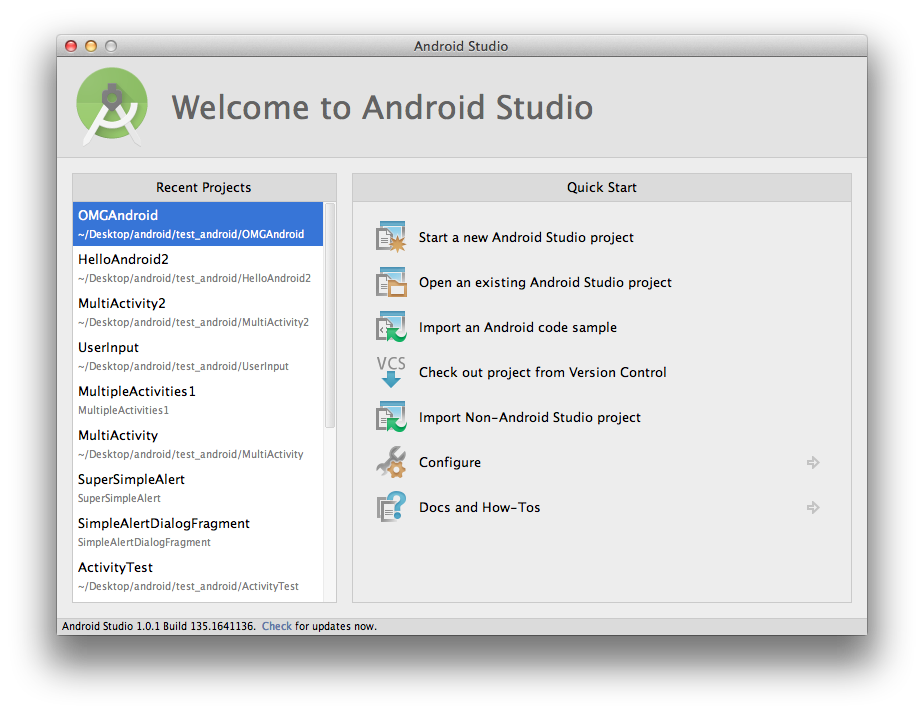
\includegraphics[width=\textwidth]{images/android-studio_01_welcome}
\caption{Android Studio welcome pane}
\label{fig:android.studio_welcome}
\end{figure}

\paragraph{} You should see the window shown in Figure \ref{fig:android.studio_config}. Enter a name for your new Application. This will also be used for your project name. For our first app let's call it `HelloNapier'. For `Company Domain' I suggest you enter `napier.ac.uk'. Now click Next to continue.

\begin{figure}[H]
\centering
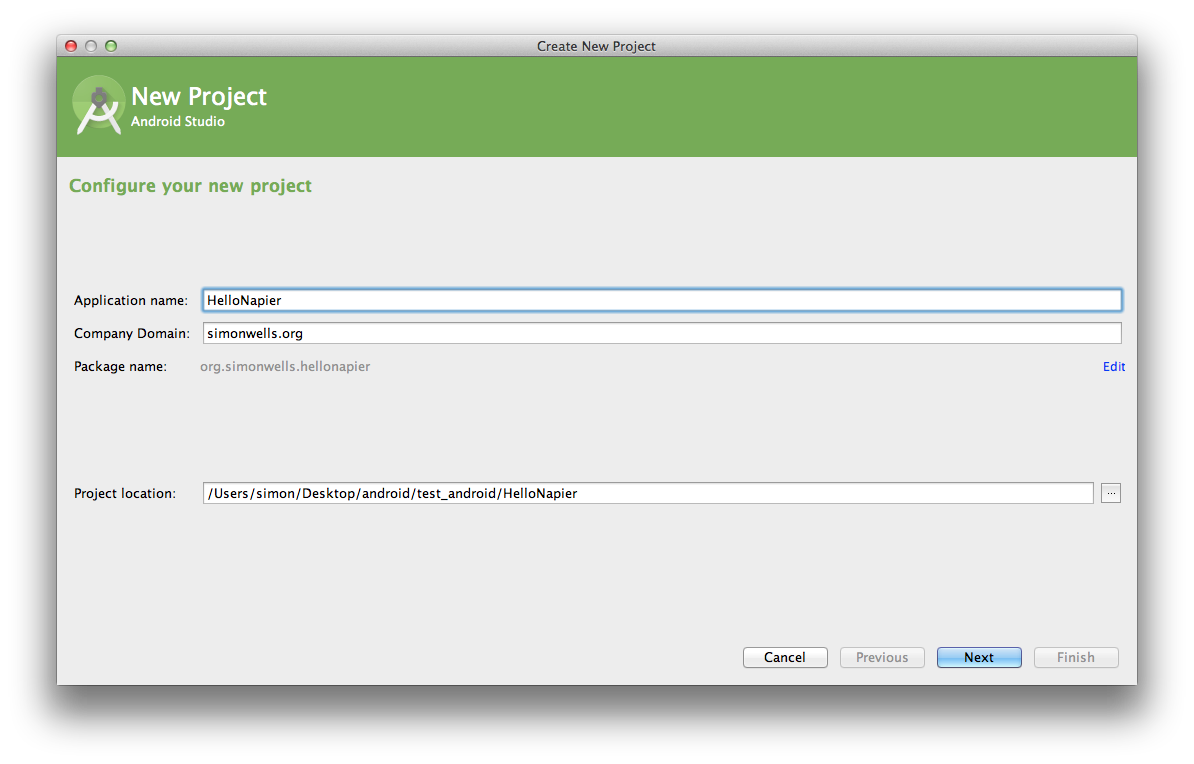
\includegraphics[width=\textwidth]{images/android-studio_02_configure}
\caption{Android Studio new app configuration pane}
\label{fig:android.studio_config}
\end{figure}

\paragraph{} On this screen, accept the defaults for now. NB. These should be as shown in Figure \ref{fig:android.studio_form}. Now click Next.

\begin{figure}[H]
\centering
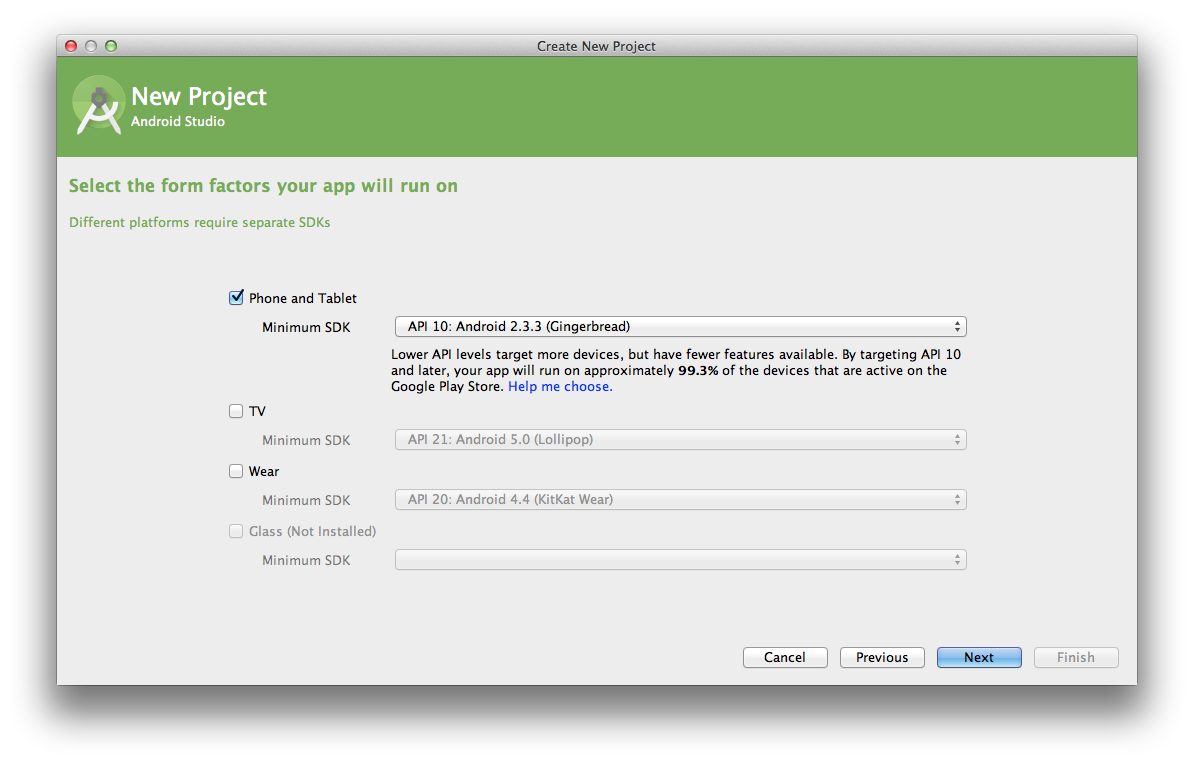
\includegraphics[width=\textwidth]{images/android-studio_03_form-factors}
\caption{Android Studio form factor selection pane}
\label{fig:android.studio_form}
\end{figure}

\paragraph{} Again, accept the default, `Blank Activity', which should be highlighted, then click Next.

\begin{figure}[H]
\centering
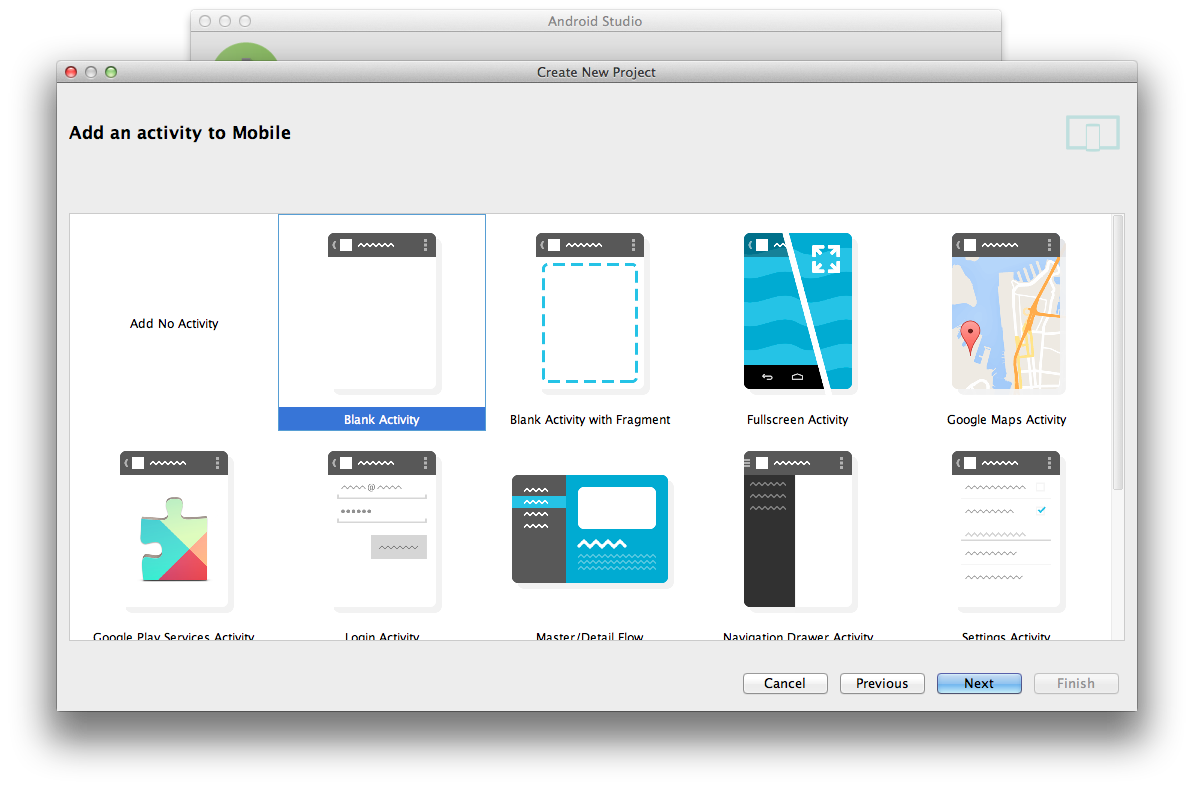
\includegraphics[width=\textwidth]{images/android-studio_06_activity}
\caption{Android Studio activity setting pane}
\label{fig:android.studio_activity}
\end{figure}

\paragraph{} Accept the defaults on this screen for now and click Next again.

\begin{figure}[H]
\centering
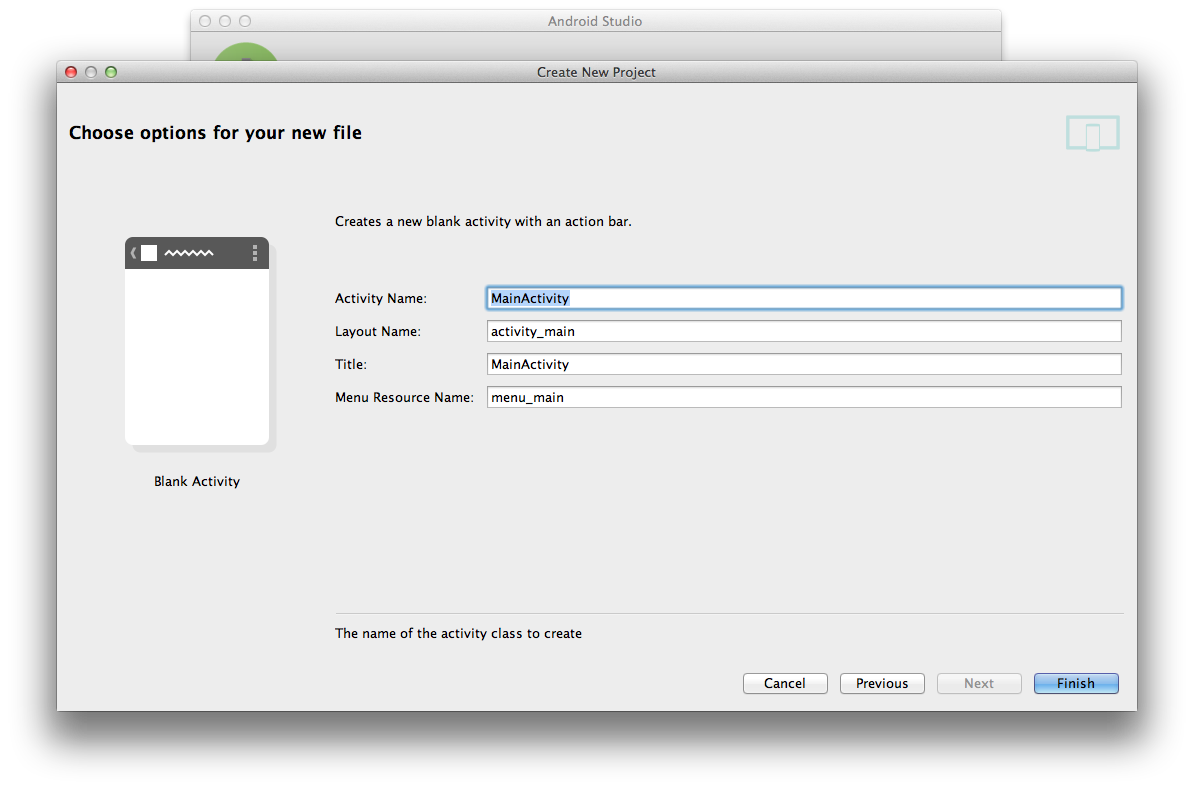
\includegraphics[width=\textwidth]{images/android-studio_07_options}
\caption{Android Studio options pane}
\label{fig:android.studio_options}
\end{figure}

\paragraph{} After a brief pause, whilst your machine loads all of the relevant libraries and creates your project file, you should be presented with the Android Studio workspace as shown in Figure \ref{fig:android.studio_studioui}.

\paragraph{NB.} It can take a while for your new project to load completely which depends upon the speed of your machine. If there are any errors or warnings on screen, especially in the preview window which renders waht your Android app interface will look like, then your project hasn't loaded completely yet.

\begin{figure}[H]
\centering
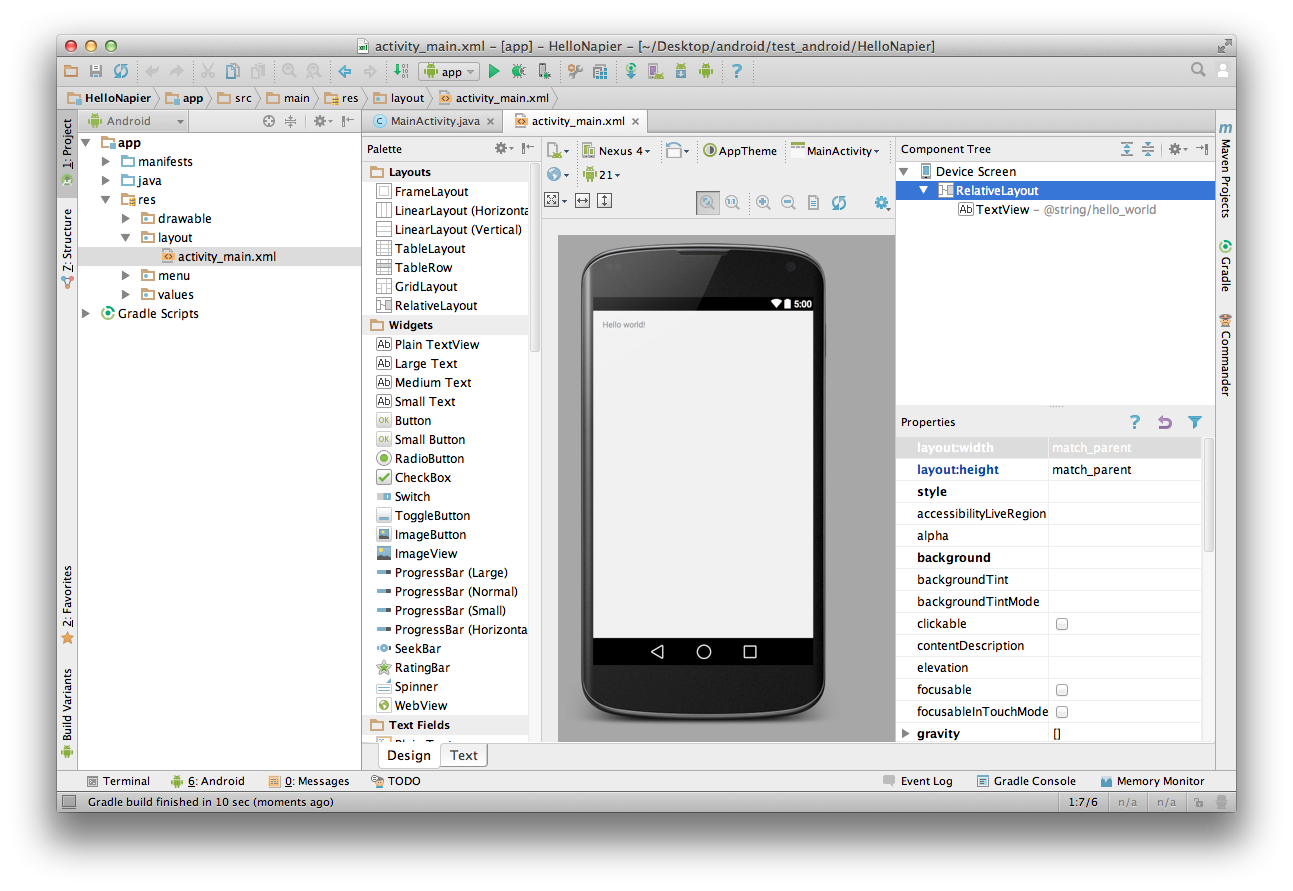
\includegraphics[width=\textwidth]{images/android-studio_08_studio-ui}
\caption{Android studio UI with default Android app}
\label{fig:android.studio_studioui}
\end{figure}

\paragraph{} Congratulations. You just created a New Android Studio projectThis process can be summarised as follows:

\begin{enumerate}
\item Click `Start a new Android Studio project'
\item Type in an application name \& Company Domain (napier.ac.uk) then click `Next'
\item Select an API level
\item Ensure `Blank Activity' is selected then click `Next'
\item Click Finish
\end{enumerate}

\paragraph{} Now you have created your first Android project. Whenever we say `Create a new project' we mean go though steps 1 to 5 ({\bf{you will have to either give each new project a different name or else save them to different locations}}).

\paragraph{} It is worth going through this process several times to become familiar with it. Once you have done it half a dozen times or so you should become comfortable with the idea of creating a new Android project and it shouldn't take more than a few seconds.

\paragraph{} It is also worth exploring some of the options that the project creation wizard offers. In particular it is worth exploring the API levels page to see what the differences are between the different API levels supported by Android. When you are on the form factors page shown in Figure \ref{fig:android.studio_form} click the link to ``Help me choose''. This will cause the API Level window to be displayed which is illustrated in Figure \ref{fig:android.studio_apilevel}.

\begin{figure}[H]
\centering
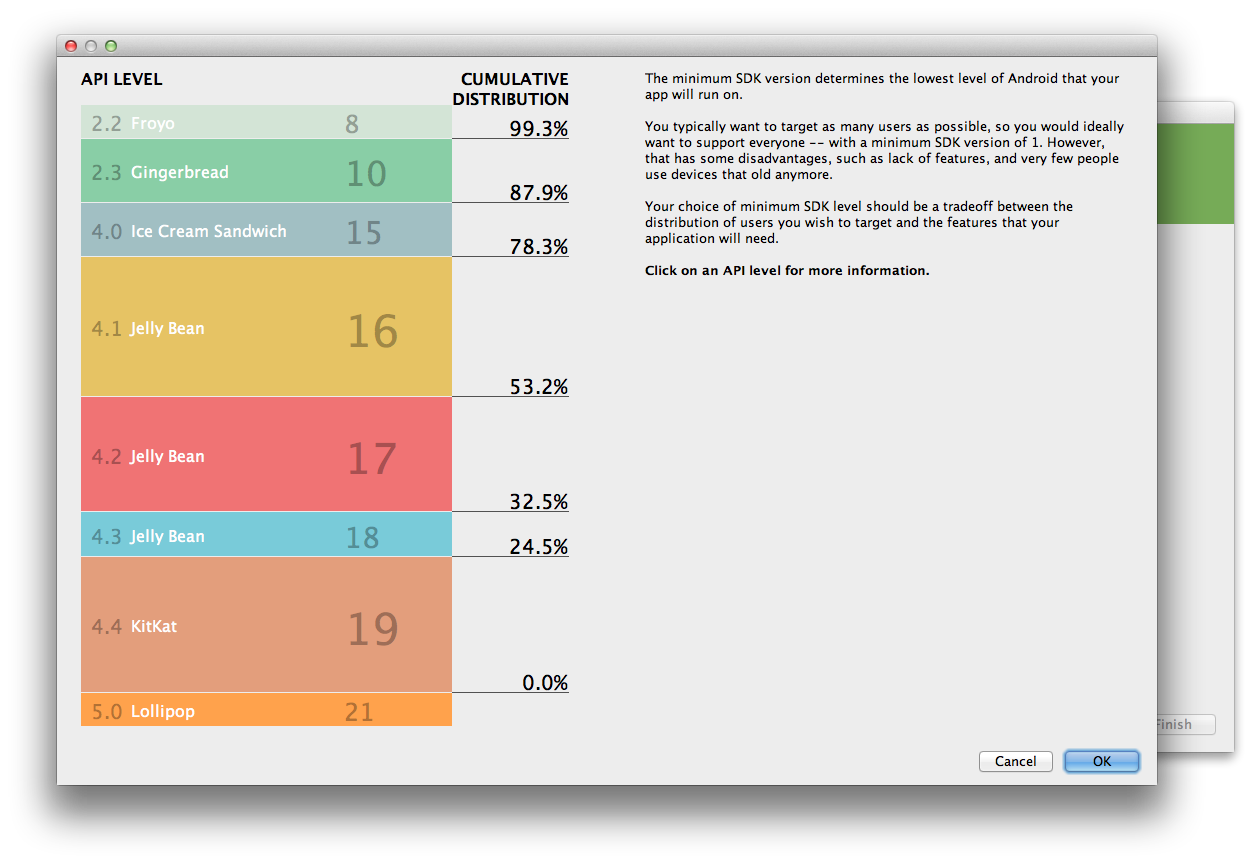
\includegraphics[width=\textwidth]{images/android-studio_04_api-level}
\caption{Android Studio API level selection screen}
\label{fig:android.studio_apilevel}
\end{figure}


\paragraph{} This page gives you an idea of the proportion of the market for Android devices that you can target with each API level. If you click on a particular level, e.g. `2.3 Gingerbread' then you will see extra information about the features offered by that verson of Android. Remember, higher API levels support newer or more refined features whereas lower levels are supported by a wider proportion of the population of Android devices. Choosing an API level is therefore partly a technical decision, because it affects what you can do, partly a business decision, because it affects the size of your potential customer base, and partly an aesthetic decision, because how things are displayed is also affected by API level. So choose wisely ;) 

\begin{figure}[H]
\centering
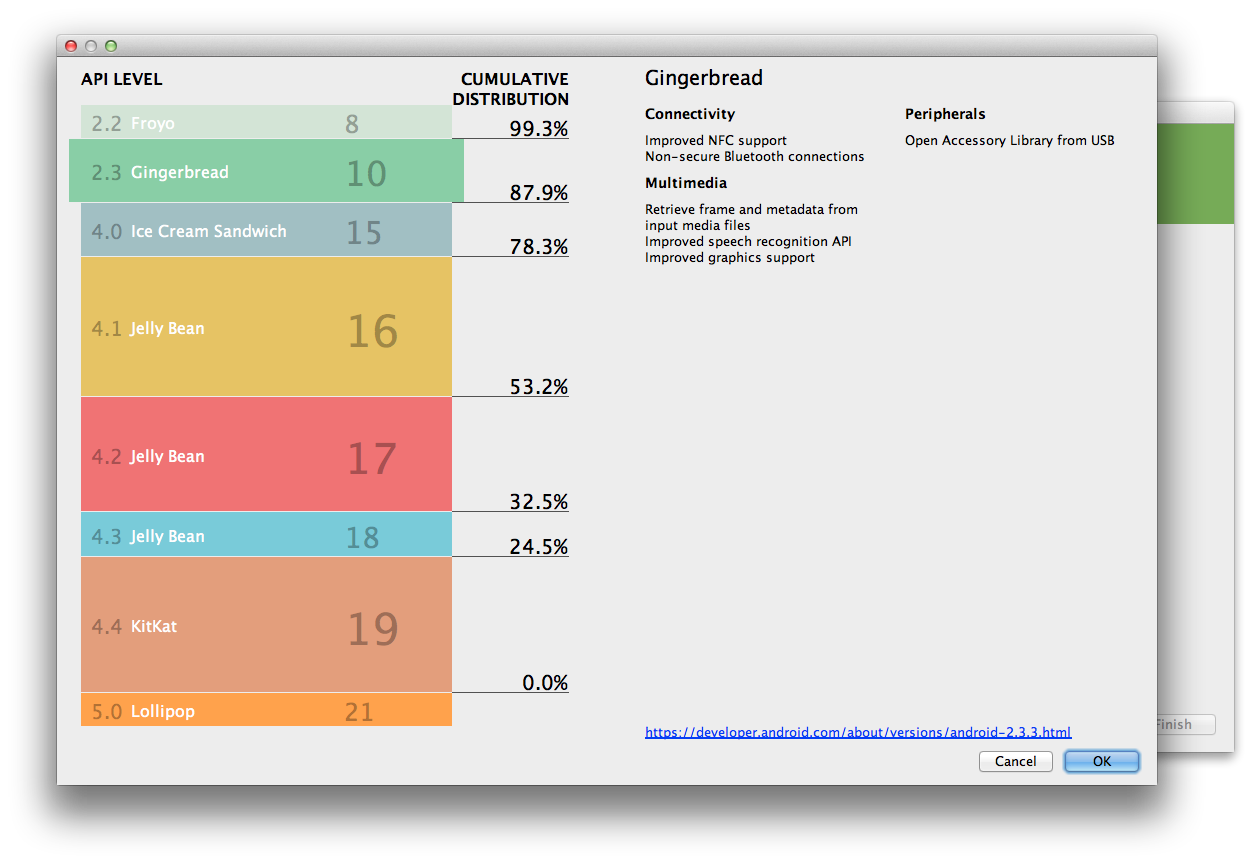
\includegraphics[width=\textwidth]{images/android-studio_05_api-level-details}
\caption{Android Studio API level details screen}
\label{fig:android.studio_apidetails}
\end{figure}

\paragraph{} It can take quite a while, even minutes, for Android Studio to completely load your new project and all of the supporting libraries. If the preview of the Android UI isn't fully displayed or has a message on it then Android Studio is still loading and compiling things so it is best to let it finish. Similarly if there are errors or warnings in the ``Problems'' tab then it is likely that these are due to your IDE still loading and building resources. Sometime the IDE can also get ahead of itself and tries to use one component before another is properly loaded. Usually when this occurs there will be a message with a link to let you reload or retry the component. When we build a new Android Studio project, especially for the first time, there will be a lot of code to generate and libraries to link, and this can take a while. Also, because everyone in the class is trying to do this at the same time, and Android Studio runs across the university network from the ``U:\'' drive there can be some significant lag. At this point you should just wait for things to resolve themselves. You imght also notice, in the status bar of Android Studio, that there is a message regarding scanning or indexing files, this happens when we first use Android Studio, it can take a while to complete, and it can cause significant performance issues initially.

\paragraph{} Now you need to build and run your app. This is important because we want to actually see our app running and doing something don't we?

\section{Running our app using Android Virtual Devices (AVDs)}
\label{avd}
\paragraph{} Because Android apps are not Windows (or Linux, or MacOS) apps they will not usually run natively on our operation systems (unless you are using Android as your OS but let's ignore that case for now). That means that you cannot just double click on your app and have it run in a window. Android apps rely on the Android OS to provide not just the platform libraries that contain all the code you didn't write but also all of the app management functionality. Android apps are a collection of activities (we will talk about these in class next week) and the OS manages when to display a given activity and when to allow another activity to take precedence. As a result we need a way to run our Android app. There are three alternatives, you can use a hardware device plugged into your computer via USB, or you can emulate the hardware of an Android device. Android devices usually run on an ARM architecure, which is different to most desktop machines, and thus that architecture needs to be emulatedin software, this can be very slow. A third option is to use a virtual device that runs a version of the Android OS that is built for the x86 architecture. This allows us to use real hardware, e.g. CPU cores and RAM, to run the Android OS in the virtual device. We can then load our Android app in this virtual version of Android and have it run with acceptable performance. This approach is known as using an `Android Virtual Device' (AVD) and we interact with AVDs through the AVD manager. We can access this through the Tools $\to$ Android $\to$ AVD Manager menu option. The AVD manager lets you set up multiple AVDs, e.g. targetting different versions of Android or simulating different hardware capabilities. For the moment we should merely use the default AVD and accept the defaults that the AVD manager suggests. Bare in mind that an AVD is quite large, around 650MB each, so you might not want to create too many of them. Currently AVDs are stored in the C: drive of the JKCC machines so each time you use a different machine you will probably have to create a new AVD. This is a known ``feature'' of the JKCC which is being worked on. 

\paragraph{} Once you have created a new Android device then it it needs to be started. As this process is essentially starting up a whole operating systems this can take a few moment. Eventually however you should see a new window that looks a bit like an Android device

\paragraph{} Once you have an AVD created you can select the Run $\to$ Run `app' menu optionand your Android app will be built and tranferred to your AVD. You might have to select the AVD that you want to run the app in from a list of running devices. NB. If you have attached a harware device to your computer using USB then this device should also be listed however there are some caveats; you will need to have the correct drivers installed for your device and this will probably not work in the JKCC with your own device but should be OK on your own laptop.

\paragraph{} That's it for this week. You should get yourself \emph{very} comfortable with these processes and go through them multiple times as every app that you will build during the mdule, and you will build tens if not hundreds of apps, will require you to set up a new project. You should only need a single AVD using the default settings for the majority of the lab exercises. If other settings are required for a particular exercise then this will be flagged as necessary. That said, experiment with Android studio, explore some of the features that it offers, and get as familar as you can with it so that you are ready to do more in subsequent labs.




\chapter{Platforms \& Lifecycles}

\section{Aims}
\paragraph{} At the end of the practical portion of this topic you will be able to:

\begin{itemize}
\item Understand the basic relationship between Android project files
\item Display text using an Android View
\item Display buttons and respond when they are used
\item Display notifications (Toasts) to users
\item Log output from your app and view it using logcat
\end{itemize}

\section{Baby-steps with Android}
\paragraph{} Create a new Android project using the process we followed for HelloAndroid. You should give your project a different name, for example, `HelloString' (because to begin with we shall be manipulating the strings that say Hello ;). It is a good idea to come up with a naming scheme for your Android projects or perhaps to organise them in folders based upon module topic or semester week number so that later in the course you can refer back to earlier code you have developed.

\paragraph{} In Android Studio open the Activity Java file. This should be called `MainActivity.java' and will be located in the 
\begin{framed}
src/uk/ac/napier/napier-id/HelloString/ 
\end{framed}
\paragraph{} folder of your project. 

\paragraph{} There isn’t a lot to see here. Most of what you see is commonly called `boilerplate' and is basically setting up the things that the Android libraries need to provide the framework for an empty project. What you will notice is that the things you see on screen when you run this app are not anywhere to be found in this Java file. This is because all the text, graphics, and layout information is created and stored in separate XML files. These XML files are then referenced from the Java code or other XML files. This means that Android has a very flexible development system which encourages well structured and reusable designs but the drawback is that it is a little complicated to get started with.

\paragraph{} There are a few things to take particular note of in the MainActivity.java file.

\begin{lstlisting}
    public class MainActivity extends Activity {
\end{lstlisting}

\paragraph{} In this line we are creating a class, called MainActivity, which inherits from the Activity parent class. Rather than creating a main method like we do in a Java program we are allowing the Android libraries to provide the main method instead. This is because we are not writing a Java program, we are writing an Android app, and these are different things. When we write an Android app we will be working within the framework of classes and libraries provided by the Android platform and there are certain requirements for an Android app to become an Android app. Because the core of an Android app is the Activity we must use the existing Android classes that provide Activity functionality. There are a number of Activity and other classes that we can inherit functionality from but for the moment we will concentrate on the core Activity class.

\paragraph{} Because we have inherited from the Activity base-class we must implement a number of methods that allow our apps functionality to `hook in' to the framework provided by the Android platform. Importantly right now we override the onCreate method. This is the method that pretty much starts the life-cycle of our app. It is called when our app is created and does a lot of work for us. In this case, with our basic HelloString app all it does is call the parent class onCreate method to ensure that the hierarchy of Activity classes are properly initialised then

\begin{lstlisting}
setContentView(R.layout.activity_main);
\end{lstlisting}

\paragraph{} Let's unpack this a little. The setContentView part is a call to a method related to displaying something on screen. We then have the argument to this method which contains 
\begin{framed}
R.layout.activity\_main
\end{framed}
\paragraph{} What this means is that we are referencing an Android resource. `R' is short for resource, notice that in package explore there is a folder called `res'. This contains all of the information about things that our can display, amongst other things. For our purposes we can consider `R' to refer to these resources. In reality it is slightly more complicated because when we build our app the contents of the res folder are assembled into a more efficient representation and the `R' file is essentially an index to our efficient representation of our resources. Going back to our line of code, without the res folder there is a sub-folder called layout, inside of which is a file called `activity\_main.xml'. This line of code is essentially saying display the layout described in activity\_main.xml, so perhaps we should take a look at that file. Use package explorer to open it.

\paragraph{} There is a lot to take in in this file. For a start. it doesn't look like a Java language source file. That is because it isn't. It is an eXtensible Markup Language (XML) file\footnote{\url{http://en.wikipedia.org/wiki/XML}}. XML is used to describe and specify Android resources. There are a number of things happening in this file. The top part

\begin{lstlisting}<RelativeLayout xmlns:android="http://schemas.android.com/apk/res/android"
    xmlns:tools="http://schemas.android.com/tools" android:layout_width="match_parent"
    android:layout_height="match_parent" android:paddingLeft="@dimen/activity_horizontal_margin"
    android:paddingRight="@dimen/activity_horizontal_margin"
    android:paddingTop="@dimen/activity_vertical_margin"
    android:paddingBottom="@dimen/activity_vertical_margin" tools:context=".MainActivity">
\end{lstlisting}

\paragraph{} basically describes a layout for the things to display on screen. Essentially telling Android to use the `Relative Layout' to organise the things that it draws and to use the parameters that are supplied e.g. layout\_height, paddingRight, paddingTop, and paddingBottom. We will see more about layouts and how to arrange things nicely on screen in the next practical so for now we will just ignore it. The next section is more interesting right now:

\begin{lstlisting}    <TextView android:text="@string/hello_world" android:layout_width="wrap_content"
        android:layout_height="wrap_content" />
\end{lstlisting}

\paragraph{} This is interesting because it is the bit that tells the Android platform to display our "Hello World" message. Again, like the use of `R' in MainActivity.java to provide flexibility we have another bit of indirection. Instead of just having all of the strings that our app uses in the place that they are used, instead we have them all collected in a single location, another resource file, called strings.xml which can be found here

\begin{framed}
res/values/strings.xml
\end{framed}

\paragraph{} {\bf{Why do you think that it might be useful to collect all of the strings together in one place?}}

\paragraph{} Our layout file contains a reference to a specific string, stored in the strings.xml resource file, which we want to be displayed onscreen in this layout. The reference is the `@string/hello\_world'. The reference uses `@string' to indicate that the string resource is in the strings.xml file then the name of the resource `hello\_world' to specify the particular string to display. Use package explorer to find and open the strings.xml file.

\begin{lstlisting}
<?xml version="1.0" encoding="utf-8"?>
<resources>

    <string name="app_name">HelloAndroid</string>
    <string name="hello_world">Hello world!</string>
    <string name="action_settings">Settings</string>

</resources>
\end{lstlisting}

\paragraph{} The string that displays the message is the one called `hello\_world'. The content of the string comes between the $<$string name="..."$>$$<$/string$>$ tags, in this cases ``Hello world!''. If you havn't done so yet. Run the project and look at the output. Then try altering the content of the string to display another message of your own design. From here you can even change the name of your app by altering the content of the `app\_name' string but we can leave that alone for now.

\paragraph{} While we have the emulator running we will try using it a bit more, the advanced features of the emulator and how we can interface with it will be covered in a later practical but you should make yourself familiar with what the various buttons on the emulator can do:
•	the home button will return you to the home screen, 
•	the menu button differs with each application and 
•	the back button acts like a browser back button. You will find that the emulator contains the majority of a basic Android phones features, exceptions include Bluetooth and camera as they would require specific hardware.
It is possible to run applications already on the emulator, including our application from earlier. Click the launcher grid button (in the centre of the home screen) and scroll through the list of existing apps, you should be able to find your app and run it from here. To add an app to the home page, press and hold the icon and when the emulator changes to the home page you can drag the icon into place and release it to place it there.

\begin{figure}[H]%[htb]
\centering
    \begin{subfigure}[b]{0.45\textwidth}
        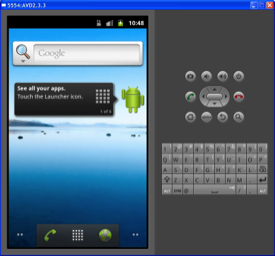
\includegraphics[width=\textwidth]{images/android_home}
        \caption{Android Home}
        \label{fig:android-home}
    \end{subfigure}
    ~ 
    \begin{subfigure}[b]{0.45\textwidth}
        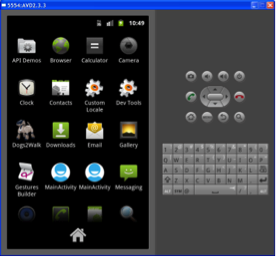
\includegraphics[width=\textwidth]{images/android_apps}
        \caption{Android Apps}
        \label{fig:android-apps}
    \end{subfigure}
\caption{Android home screen \& apps}
\label{fig:android-home-apps}
\end{figure}

\section{The DateTime App}
\paragraph{}Now we have an understanding of how the applications are built and executed on the emulator we will build our first application that does something more than just display the Hello message. Along the way we will explore some of the basic user interface controls available on the Android platform. On Android anything that can be displayed on screen is called a View and this includes all of those elements that we are used to on other platforms that we usually refer to as GUI widgets.

\paragraph{} We're going to create an app which displays the current date and time when you click a button. Create a new app and call it `DateTime'. Open the graphical layout - one way of doing this is simply to double click the activity\_main.xml file in the res/layout folder. You can delete the HelloWorld message, just select it with the mouse and delete it, as we won't be using it.

Your should see an area of the Android Studio UI which provides a `Palette' or `toolbox' of graphical widgets that you can use in your app. Drag a textview view from the palette onto the AndroidApp activity layout. Notice that the graphical layout is a good way to place and arrange Android views on screen to rapidly create a GUI. Select the new Text View – then change the Text property to ``DateTime'' (without the quotes) and the name to ``TextView1''. Click now on the activity\_main.xml tab to see what has happened to the XML code – you should now have a block called <EditText...> like so

\begin{lstlisting}
<TextView
        android:layout_width="wrap_content"
        android:layout_height="wrap_content"
        android:text="DateTime"
        android:id="@+id/textView1"
        android:layout_below="@+id/button1"
        android:layout_centerHorizontal="true" />
\end{lstlisting}

\paragraph{} Now return to graphical layout and select Form Widgets. Drag a button over to your activity layout.  Right click (or double click in Android Studio) to edit the text that goes onto the button - and select Edit Text. You can enter the new text in the field at the bottom (under New String...). Change to ``Click me!''. The default name for your button is button1 – check this by clicking on the button then looking at the properties.

\begin{lstlisting}
<Button
        android:layout_width="wrap_content"
        android:layout_height="wrap_content"
        android:text="Click Me!"
        android:id="@+id/button1"
        android:layout_centerHorizontal="true"
        android:layout_marginTop="79dp"
        android:layout_centerVertical="true" />
\end{lstlisting}

\paragraph{} So we now have a text box and we have a button. Check your app now – select the project from the Package Explorer then click the play button (a green `play' triangle on the menu bar):

\paragraph{} The problem now is that our app doesn't actually do anything. The Click Me! button has no functionality and the TextView will just display DateTime forever. We need to write some code to do something when the button is clicked. We’re going to overwrite the DateTime string with the actual date and time. How are we going to do this? Well, we need to have a handler that will listen for button clicks, we need to write a little bit of code to get the current time and date, and we need a little bit of code to update the TextView with our new time and date.

\paragraph{} Open MainActivity.java. First we need to add some imports so that our app can access the libraries that it needs to do our extra functionality. By default the basic app project only has the minimal set of imports that it needs to display the Hello World message. We have to add other imports to do different things. These are the imports that we need in MainActivity.java in addition to the ones that are already there:

\begin{lstlisting}
import android.view.View;
import android.view.View.OnClickListener;
import android.widget.Button;
import android.widget.TextView;
import java.util.Date;
\end{lstlisting}

\paragraph{} Now we need to add some code to the onCreate method:

\begin{lstlisting}
Button btn1 = (Button) findViewById(R.id.button1);
        btn1.setOnClickListener(new OnClickListener() {
            @Override
            public void onClick(View v) {
                TextView tv1 = (TextView) findViewById(R.id.textView1);
                tv1.setText(new Date().toString());
            }
        });
\end{lstlisting}

\paragraph{} You should now be able to run your app and each time you click the button you will see an updated date and time displayed in the TextView.

\paragraph{} Just for completion. Open the strings.xml file for your app and add a new string resource to represent the text of your button, e.g.

\begin{lstlisting}
<string name="button1">Click Me!</string>
\end{lstlisting}

\paragraph{} Now, in your activity\_main.xml, update the entry for the button to reference the string resource rather than embedding the string directly in the activity, e.g.

\begin{lstlisting}
android:text="@string/button1"
\end{lstlisting}

\paragraph{} Now try to do the same for the TextView. Add a string resource for the default content of the TextView then reference that string resource from activity\_main.xml

\paragraph{} You should now experiment with the various settings that you can use for TextViews and Buttons. Try adding a text view or more buttons and changing the text on them rather than the text on the button being pressed. Use the graphical designer to drag and drop various views onto your activity and use the property inspector to set various properties for the views. Remember to frequently run your app after you have made even small changes to see what effect they have. You should also frequently compare the visual view of the activity which gives you an idea of how the app will look with the contents of the activities XML file. The aim of this is to get a feel for the various widgets that are available, the settings that they can have, and how the views are actually represented as resources in the XML files of your app.

\section{Toasts}
\paragraph{} A toast\footnote{There is more general information about Toasts available at the Android website \url{http://developer.android.com/guide/topics/ui/notifiers/toasts.html} as wells developer documentation \url{developer.android.com/reference/android/widget/Toast.html}} is a view that contains a quick message or notification to the user, the Toast class helps you create and show Toast messages without having to set up the View in a layout file. When the View is shown to the user it appears to float over the current application activity, it never receives focus over and it will not interrupt the users current actions like typing. Examples of common Toast messages are the volume control or save messages when you save a draft of a text message. The idea is to be as unobtrusive as possible while showing important information to the user.

\paragraph{} We can adapt our DateTime app to display a toast each time we click the button. This will illustrate how you can integrate toasts into your own apps. In MainActivity.java we need an import for the Toasts class:

\begin{lstlisting}
import android.widget.Toast;
\end{lstlisting}

\paragraph{} Having imported the Toast class we can use it, which is pretty straightforward. In the onClick handler that we created earlier for our button, just add the following after the call to setText on our TextView

\begin{lstlisting}
Toast.makeText(MainActivity.this, tv1.getText(),Toast.LENGTH_LONG).show();
\end{lstlisting}

\paragraph{} Toasts are also a useful way to do quick output if you want to just check the value of something during development. However there is also a much better way....

\section{Logging}
\paragraph{} Logging\footnote{Developer documentaiton available here \url{http://developer.android.com/reference/android/util/Log.html}} is really important once you start to build larger apps. Because Android doesn't have a console or terminal which our app can output messages to we need something else. We could add widgets into our GUI to let us quickly see the values that our apps hold but this is far from ideal. The logging subsystem is designed to enable you to output data from your app outside of the graphcial views that make up your app.

\paragraph{} Android Studio has areas set aside to display logs whilst you are developing and running your apps. These are in the logcat area and will display both log messages that you cause to be sent from your code, as well as log messages that arise due to errors during runtime.

\paragraph{} To use logging we need some imports again in MainActivity.java

\begin{lstlisting}
import android.util.Log;
\end{lstlisting}

then to cause a line to be written to the log we just need a line like the following (place it in the onClick listener for your button to try it out):

\begin{lstlisting}
Log.i("org.simonwells.datetime","Button pressed");
\end{lstlisting}

\paragraph{} Notice that there are two arguments, the first is our namespace, which you should have set to match either your personal domain name, if you have one, or something like `uk.ac.napier.xx1234' if you created one based on your Napier ID. The second argument is the actual string to write into the log. You could write a static string here as we have done above with `Button pressed' or else you can build the string to display, e.g. including the id of the concerned view so that you can identify exactly which view caused the log line to be created. This is especially useful as your apps get bigger and involve more views (and more things that could go wrong).

\paragraph{} When you run your app and press the button you should see a line similar to the following in logcat:

\begin{framed}
{\scriptsize{
01-21 14:29:21.654 23977-23977/org.simonwells.datetime I/org.simonwells.datetime: Button pressed
}}
\end{framed}

\section{Summary}
\paragraph{} In this practical we have 

\begin{itemize}
\item Investigated the relationship between Android project files made up of Java source files, XML files and others.
\item Displayed text using an Android View
\item Displayed buttons and responded when they have been used
\item Displayed notifications (Toasts) to users
\item Logged output from our apps and viewed it using logcat
\end{itemize}





\chapter{Working with Activities \& User Interfaces}

\section{Aims}
\paragraph{} At the end of the practical portion of this topic you will be able to:

\begin{itemize}
\item Work with Android Activities
\item Work with user input views
\end{itemize}

\section{Activities}
\paragraph{} We will start the lab by working with activities. Remember that an activity is essentially a window that contains some user interface elements and that an app can have zero or more activities. In HelloAndroid we got a single activity by default that we used to display some views. However, using multiple activities and switching between them can be a useful way to organise your app if you want your user to navigate between multiple screens. So in this part of the lab we will look at creating activities, displaying them, and navigating between them.


\subsection{Creating}
\paragraph{} Creating new activities is straightforward if you are working in Android Studio as it provides helper wizards to add the new code for you. For example, if in the studio interface you right click on the app folder in the project explorer then select ``New'' $>$ ``Activity'' $>$ ``Blank Activity'' and call it `MainActivity2' then studio will add in the necessary code to support your new MainActivity2. This includes a java src file called `MainActivity2.java', an XML activity file called `activity\_main\_activity2.xml', an entry in the AndroidManifest.xml file, and an entry in the strings.xml file.

\paragraph{} But to really get a feel for what is happening we need to do the job by hand. Create a new android project and test that it runs. Add a new Java src file called MainActivity2.java into the same directory as MainActivity.java and edit it as follows:

\begin{lstlisting}
package org.simonwells.multipleactivities1;

import android.support.v7.app.ActionBarActivity;
import android.os.Bundle;
import android.view.Menu;
import android.view.MenuItem;


public class MainActivity2 extends ActionBarActivity {

    @Override
    protected void onCreate(Bundle savedInstanceState) {
        super.onCreate(savedInstanceState);
        setContentView(R.layout.activity_main);
    }


    @Override
    public boolean onCreateOptionsMenu(Menu menu) {
        // Inflate the menu; this adds items to the action bar if it is present.
        getMenuInflater().inflate(R.menu.menu_main, menu);
        return true;
    }

    @Override
    public boolean onOptionsItemSelected(MenuItem item) {
        // Handle action bar item clicks here. The action bar will
        // automatically handle clicks on the Home/Up button, so long
        // as you specify a parent activity in AndroidManifest.xml.
        int id = item.getItemId();

        //noinspection SimplifiableIfStatement
        if (id == R.id.action_settings) {
            return true;
        }

        return super.onOptionsItemSelected(item);
    }
}
\end{lstlisting}
\paragraph{} Compare the code in MainActivity.java to that in MainActivity2.java, how do they differ? What does this tell you?

\paragraph{} Now create a corresponding layout for MainActivity2. In res/layout create a new xml file called `activity\_main2.xml' and edit it as follows:

\begin{lstlisting}
<RelativeLayout xmlns:android="http://schemas.android.com/apk/res/android"
    xmlns:tools="http://schemas.android.com/tools" android:layout_width="match_parent"
    android:layout_height="match_parent" android:paddingLeft="@dimen/activity_horizontal_margin"
    android:paddingRight="@dimen/activity_horizontal_margin"
    android:paddingTop="@dimen/activity_vertical_margin"
    android:paddingBottom="@dimen/activity_vertical_margin" tools:context=".MainActivity">

    <TextView android:text="@string/activity2_name" android:layout_width="wrap_content"
        android:layout_height="wrap_content" />

</RelativeLayout>
\end{lstlisting}

\paragraph{} Again, compare activity\_main2.xml to activity\_main.xml and notice the differences between them. Why do you think we did this? Actually, in this case we could have kept the layout file identical but we need a way to differentiate between them once they run, that is why the text references a different string resource.

\paragraph{} That is the bulk of the work necessary to create a new activity. However we are not quite ready to run out app yet. Open strings.xml and add the following to it:

\begin{lstlisting}
<string name="activity2_name">ACTIVITY TWO!!!!???!!</string>
\end{lstlisting}

\paragraph{} Now open you AndroidManifest.xml and add the following below the existing </activity>:

\begin{lstlisting}
        <activity
            android:name=".MainActivity2"
            android:label="@string/app_name" >
        </activity>
\end{lstlisting}

\paragraph{} Your AndroidManifest.xml should now look like this:

\begin{lstlisting}
<?xml version="1.0" encoding="utf-8"?>
<manifest xmlns:android="http://schemas.android.com/apk/res/android"
    package="org.simonwells.multipleactivities1" >

    <application
        android:allowBackup="true"
        android:icon="@drawable/ic_launcher"
        android:label="@string/app_name"
        android:theme="@style/AppTheme" >
        <activity
            android:name=".MainActivity"
            android:label="@string/app_name" >
            <intent-filter>
                <action android:name="android.intent.action.MAIN" />

                <category android:name="android.intent.category.LAUNCHER" />
            </intent-filter>
        </activity>
        <activity
            android:name=".MainActivity2"
            android:label="@string/app_name" >
        </activity>
    </application>

</manifest>
\end{lstlisting}

\paragraph{} That is all that is needed to create a new Activity. Two new files, a java source file and an XML layout file, and a couple of edits to make sure that your app knows about the new stuff. You can now run your app.

\paragraph{} Hmmm. Not much difference there? Why do you think that is? 

\paragraph{} Lets edit our AndroidManifest.xml to display the new Activity instead of the default one. To do this we need to add an $<$intent-filter$>$ to our $<$activity$>$ section for the new activity and remove it from the old one, e.g.

\begin{lstlisting}
<intent-filter>
                <action android:name="android.intent.action.MAIN" />

                <category android:name="android.intent.category.LAUNCHER" />
            </intent-filter>
\end{lstlisting}

\paragraph{} So your edited AndroidManifest.xml should look like this:

\begin{lstlisting}
<?xml version="1.0" encoding="utf-8"?>
<manifest xmlns:android="http://schemas.android.com/apk/res/android"
    package="org.simonwells.multipleactivities1" >

    <application
        android:allowBackup="true"
        android:icon="@drawable/ic_launcher"
        android:label="@string/app_name"
        android:theme="@style/AppTheme" >
        <activity
            android:name=".MainActivity"
            android:label="@string/app_name" >

        </activity>
        <activity
            android:name=".MainActivity2"
            android:label="@string/app_name" >
            <intent-filter>
                <action android:name="android.intent.action.MAIN" />

                <category android:name="android.intent.category.LAUNCHER" />
            </intent-filter>
        </activity>
    </application>

</manifest>
\end{lstlisting}

\paragraph{} Now run your app. You should now see the second Activity displayed. You can tell the difference because instead of the ``Hello world!'' message you should see the ``ACTIVITY TWO!!!!???!!'' message. But this isn't really good enough. We can't edit the app's manifest file every time we want to create a new Activity.

\subsection{Starting}
\paragraph{} Create a new Android project to include three activity classes. Up until now we have only been using a single Activity in our applications, now we will be using multiple Activity classes we will need a way to start them. We do this through launching an “intent” and passing in the name of the activity you want to start. Check out http://developer.android.com/guide/topics/fundamentals.html for more information on Intents. Below is some simple code that will start an Activity on a Button click:

\begin{lstlisting}
Button button1 = (Button) findViewById(R.id.button1);
button1.setOnClickListener(new OnClickListener() {
	public void onClick(View v) {
		Intent activityA = new Intent(MainActivity.this, ActivityA.class);
		startActivity(activityA);
	}
});
\end{lstlisting}

\paragraph{} Now create a new class in your project – call it ActivityA. It doesn’t have to do anything in particular, for example – this one just displays a toast so you know you’re now in ActivityA:

\begin{lstlisting}
package com.example.w4p2;

import android.app.Activity;
import android.os.Bundle;
import android.widget.Toast;

public class ActivityA extends Activity {
	public void onCreate(Bundle savedInstanceState) {
		super.onCreate(savedInstanceState);
		setContentView(R.layout.activity_a); //You'll need to create a layout named activity_a
		
		Toast.makeText(getBaseContext(), "In Activity A", Toast.LENGTH_LONG).show();
		//Navigation back is via phones back button
	}
}
\end{lstlisting}

\paragraph{} Then add it to your android manifest file (which says what makes up your project).

\begin{lstlisting}
<?xml version="1.0" encoding="utf-8"?>
<manifest xmlns:android="http://schemas.android.com/apk/res/android"
    package="com.example.w4p2"
    android:versionCode="1"
    android:versionName="1.0" >

    <uses-sdk
        android:minSdkVersion="8"
        android:targetSdkVersion="17" />

    <application
        android:allowBackup="true"
        android:icon="@drawable/ic_launcher"
        android:label="@string/app_name"
        android:theme="@style/AppTheme" >
        <activity
            android:name="com.example.w4p2.MainActivity"
            android:label="@string/app_name" >
            <intent-filter>
                <action android:name="android.intent.action.MAIN" />

                <category android:name="android.intent.category.LAUNCHER" />
            </intent-filter>
        </activity>
        <activity android:name="ActivityA" />
        <activity android:name="ActivityB" />
    </application>
</manifest>
\end{lstlisting}

\paragraph{} Now add a second activity – B – just to try it all out. What if we need to get data back from this new activity? The best way is to use a different method: startActivityForResult (activityA, 1);
So we launch the activity then what? We need a handler to call when our activity has completed. Add this code in your main activity:

\begin{lstlisting}
protected void onActivityResult(int requestCode, int resultCode, Intent data) {
    	//Check which request we're responding to - only 1!
    	if (requestCode == 1) {
    		//Make sure request was successful
    		if (resultCode == 1) {
    			String returnString = data.getStringExtra("String");
    			Toast.makeText(getBaseContext(), "In main and string returned = " + returnString, Toast.LENGTH_SHORT).show();
    		}
    	}
}
\end{lstlisting}

\paragraph{} And what does the activity you launch look like now? We have to get the data packaged up as we expect to receive it:

\begin{lstlisting}
String stringToReturn = "Sally Smith";
        Intent returnIntent = new Intent();
        returnIntent.putExtra("String", stringToReturn);
        setResult(1, returnIntent);
        finish();
\end{lstlisting}

\paragraph{} Have a go! If you get stuck ask!

%\subsection{Managing Multiple Activities}
%\paragraph{} Rather than creating a new activity for every screen in your app, it make sense to reuse resources when appropriate. For example, if your user is presented with a list of items that can be displayed, you could either have an activity for each item and switch between them after user interaction, or a single activity, designed to display your items consistently, which is reused based on user interaction. Having less activities, but reusing them in a sensible manner can help to stop your app from becoming unmanageable.


%\section{ViewGroups \& Layouts}
%\paragraph{}


\section{More Views: User Input}
\paragraph{} Remember, views are widgets that have an appearance onscreen. So user input widgets, such as text inputs, can use views just as output does. Let's explore some user input.

\paragraph{} Create a new project and check that it runs properly. Now delete the Hello World TextView so that we have an empty layout to play with.

\paragraph{} Add a ScrollView such as the following to your layout:

\begin{lstlisting}
<ScrollView
        android:layout_width="wrap_content"
        android:layout_height="wrap_content"
        android:id="@+id/scrollView"
        android:layout_centerVertical="true"
        android:layout_alignParentLeft="true"
        android:layout_alignParentStart="true"
        android:layout_marginLeft="42dp"
        android:layout_marginStart="42dp" >

        </ScrollView>
\end{lstlisting}

\paragraph{} Your activity\_main.xml should look similar to the following:

\begin{lstlisting}
<RelativeLayout xmlns:android="http://schemas.android.com/apk/res/android"
    xmlns:tools="http://schemas.android.com/tools" android:layout_width="match_parent"
    android:layout_height="match_parent" android:paddingLeft="@dimen/activity_horizontal_margin"
    android:paddingRight="@dimen/activity_horizontal_margin"
    android:paddingTop="@dimen/activity_vertical_margin"
    android:paddingBottom="@dimen/activity_vertical_margin" tools:context=".MainActivity">

    <ScrollView
        android:layout_width="wrap_content"
        android:layout_height="wrap_content"
        android:id="@+id/scrollView"
        android:layout_centerVertical="true"
        android:layout_alignParentLeft="true"
        android:layout_alignParentStart="true"
        android:layout_marginLeft="42dp"
        android:layout_marginStart="42dp" >
         
    </ScrollView>

</RelativeLayout>
\end{lstlisting}
\paragraph{} Don't worry if everything isn't \emph{exactly} the same. The graphical editor in Android Studio will sometimes try to be helpful and add extra parameters to give you a better layout.

\paragraph{} Now add a LinearLayout as a child of the ScrollView:

\begin{lstlisting}
<LinearLayout
            android:orientation="vertical"
            android:layout_width="fill_parent"
            android:layout_height="fill_parent"
            android:layout_below="@+id/scrollView"
            android:layout_centerHorizontal="true">
</LinearLayout>
\end{lstlisting}

\paragraph{} So you should end up with something like the following:

\begin{lstlisting}
<RelativeLayout xmlns:android="http://schemas.android.com/apk/res/android"
    xmlns:tools="http://schemas.android.com/tools" android:layout_width="match_parent"
    android:layout_height="match_parent" android:paddingLeft="@dimen/activity_horizontal_margin"
    android:paddingRight="@dimen/activity_horizontal_margin"
    android:paddingTop="@dimen/activity_vertical_margin"
    android:paddingBottom="@dimen/activity_vertical_margin" tools:context=".MainActivity">

    <ScrollView
        android:layout_width="wrap_content"
        android:layout_height="wrap_content"
        android:id="@+id/scrollView"
        android:layout_centerVertical="true"
        android:layout_alignParentLeft="true"
        android:layout_alignParentStart="true"
        android:layout_marginLeft="42dp"
        android:layout_marginStart="42dp" >

        <LinearLayout
            android:orientation="vertical"
            android:layout_width="fill_parent"
            android:layout_height="fill_parent"
            android:layout_below="@+id/scrollView"
            android:layout_centerHorizontal="true">

        </LinearLayout>

    </ScrollView>

</RelativeLayout>
\end{lstlisting}

\paragraph{} Neither of these elements, the ScrollView or LinearLayout do much visually. If you run the app now there isn't much to see. But they are containers which will help us to have a nice screen when we add the views in a few moments. For now, notice how the pair of $<$LinearLayout$>$ $<$/LinearLayout$>$ tags are children of, or come between, the $<$ScrollView$>$ $<$/ScrollView$>$ tags. We will deal with Layouts more in next weeks practical but for now just think of them as containers that holds views for you and automatically arrange them for you. All the ScrollView does is make its child view scrollable when the view won't fit on screen. A ScrollView can only have one child, which is our LinearLayout, but the child of the ScrollView can contain multiple further views. Lets try that out.

\paragraph{} Add three TextViews and three EditTexts to your layout so that you have three pairs of TextView then EditText, e.g. TextView, EditView, TextView, EditView, TextView, EditView in a column down the screen. Make sure to give each TextView and EditView an id so that you can reference each individually.Add strings for your TextViews to display so that the first TextView is the user's name, second is email address, and third is password.

\paragraph{} Your layout should now look similar to this:

\begin{lstlisting}
<RelativeLayout xmlns:android="http://schemas.android.com/apk/res/android"
    xmlns:tools="http://schemas.android.com/tools" android:layout_width="match_parent"
    android:layout_height="match_parent" android:paddingLeft="@dimen/activity_horizontal_margin"
    android:paddingRight="@dimen/activity_horizontal_margin"
    android:paddingTop="@dimen/activity_vertical_margin"
    android:paddingBottom="@dimen/activity_vertical_margin" tools:context=".MainActivity">

    <ScrollView
        android:layout_width="wrap_content"
        android:layout_height="wrap_content"
        android:id="@+id/scrollView"
        android:layout_centerVertical="true"
        android:layout_alignParentLeft="true"
        android:layout_alignParentStart="true"
        android:layout_marginLeft="42dp"
        android:layout_marginStart="42dp" >

        <LinearLayout
            android:orientation="vertical"
            android:layout_width="fill_parent"
            android:layout_height="fill_parent"
            android:layout_below="@+id/scrollView"
            android:layout_centerHorizontal="true">

            <TextView
                android:layout_width="wrap_content"
                android:layout_height="wrap_content"
                android:textAppearance="?android:attr/textAppearanceLarge"
                android:text="@string/name"
                android:id="@+id/tv1" />

            <EditText
                android:layout_width="match_parent"
                android:layout_height="wrap_content"
                android:id="@+id/et1"
                 />

            <TextView
                android:layout_width="wrap_content"
                android:layout_height="wrap_content"
                android:textAppearance="?android:attr/textAppearanceLarge"
                android:text="@string/email"
                android:id="@+id/tv2"
                 />

            <EditText
                android:layout_width="match_parent"
                android:layout_height="wrap_content"
                android:id="@+id/et2"
                android:inputType="textEmailAddress"
                 />

            <TextView
                android:layout_width="wrap_content"
                android:layout_height="wrap_content"
                android:textAppearance="?android:attr/textAppearanceLarge"
                android:text="@string/pw"
                android:id="@+id/tv3"
                 />

            <EditText
                android:layout_width="match_parent"
                android:layout_height="wrap_content"
                android:id="@+id/et3"
                android:password="true" />

        </LinearLayout>

    </ScrollView>

</RelativeLayout>

\end{lstlisting}

\paragraph{} Your strings.xml should look similar to this:

\begin{lstlisting}
<?xml version="1.0" encoding="utf-8"?>
<resources>

    <string name="app_name">UserInput</string>
    <string name="hello_world">Hello world!!!!</string>
    <string name="action_settings">Settings</string>
    <string name="name">Name</string>
    <string name="email">Email Address</string>
    <string name="pw">Password</string>

</resources>
\end{lstlisting}

\paragraph{} All other files in your project should be unchanged for now as we have only edited the layour and strings files, so try running your app now. You might want to futher adjust how things look. It is worth taking the time to do that now as this builds your experience of how Android apps work. When you run the app you should be able to input text into the three EditTexts. The password field should hide letters as you type them in. This behaviour is controlled by the following parameter of the EditText: 

\begin{lstlisting}
android:password="true"
\end{lstlisting}

\paragraph{} You should experiment with the other parameters that EditText, and other views have as you explore the Android platform features.

\paragraph{} Now lets consider doing something with the text entered into the EditText fields. Lets add some features to ensure that the name field is limited to a set number of characters in length and only allows names in upper-case. Open MainActivity.java and add the following code to the OnCreate method after the call to setContentView():

\begin{lstlisting}
    EditText nameTxt = (EditText) findViewById(R.id.et1);
    nameTxt.setFilters(new InputFilter[] {
        new InputFilter.LengthFilter(10),
        new InputFilter.AllCaps()
    });
\end{lstlisting}

\paragraph{} All this is doing is creating a variable, called nameTxt, that is associated with the EditText names et1. We have then used some built in classes to set some filters on the EditText, one of which limits the length of input to 10 chars, and the other which enforces upper-case. Run your app and try it out.

\paragraph{} Now lets do somethings a bit more advanced. Lets check the content of the supplied password to see whether it passes muster. For example, lets assume that the supplied password must contain a mixture of letters and numbers. A simple way to do this is to add a button which, when clicked, will take the text in the password field and tell us whether it is valid. So, add a button to your layout, inside the LinearLayout and after the last EditText:

\begin{lstlisting}
<Button
        android:layout_width="wrap_content"
        android:layout_height="wrap_content"
        android:text="@string/go"
        android:id="@+id/btn1"
        android:layout_below="@+id/scrollView"
        android:layout_centerHorizontal="true" />
\end{lstlisting}

\paragraph{} and add its content to the strings.xml e.g.

\begin{lstlisting}
<string name="go">GO!</string>
\end{lstlisting}

\paragraph{} You can run your app now and the button will be visible but it won't do anything because we haven't given it a handler to response to click events. So lets do that, add the following code to the OnCreate method of MainActivity.java after your code that added the input filters to the name field.

\begin{lstlisting}
final EditText pwfield = (EditText) findViewById(R.id.et3);
    Button go_button = (Button) findViewById(R.id.btn1);
    go_button.setOnClickListener(new View.OnClickListener() {
        @Override
        public void onClick(View v) {
            String text = pwfield.getText().toString();

            boolean valid = true;
            boolean hasNumbers = false;
            boolean hasLetters = false;

            for (int i=0; i<text.length(); i++) {
                char x = text.charAt(i);
                if (Character.isDigit(x)){
                    hasNumbers = true;
                }
                else if (Character.isLetter(x)) {
                    hasLetters = true;
                }
                else {
                    valid = false;
                    break;
                }
                if (valid && hasLetters && hasNumbers) {
                    Toast.makeText(getBaseContext(), "Password " + text + " is valid.", Toast.LENGTH_SHORT).show();
                }
                else {
                    Toast.makeText(getBaseContext(), "Password " + text + " is not valid.", Toast.LENGTH_SHORT).show();
                }

            }
        }

    });
\end{lstlisting}

\paragraph{} Most of this is normal Java. You should try to read the code to ensure that you understand exactly what is happening and why.

\paragraph{FURTHER EXERCISE} Try to add a handler for the email field which ensure that the supplied email address is correctly formatted. If you are unsure what constitutes a valid email address then it might be worth finding out more\footnote{\begin{itemize}\item Wikipedia Email Address Page: \url{http://en.wikipedia.org/wiki/Email_address} \item RFC5321 \url{http://tools.ietf.org/html/rfc5321} \item StackOverlfow discussion: \url{http://stackoverflow.com/questions/6119722/how-to-check-edittexts-text-is-email-address-or-not}\end{itemize}}.


\section{Summary}
\paragraph{} In this practical we have 

\begin{itemize}
\item Learnt about Activities
\item Worked with user input
\end{itemize}




%%%%%%%%%%%%%%%%%
%%%%%%%%%%%%%%%%%
% CASE STUDIES 
%%%%%%%%%%%%%%%%%
%%%%%%%%%%%%%%%%%


\begin{comment}
\part{Case Studies}
\chapter{Daybook}
\label{daybook}
\paragraph{}
\end{comment}

%%%%%%%%%%%%%%%%%
%%%%%%%%%%%%%%%%%
% APPENDICES 
%%%%%%%%%%%%%%%%%
%%%%%%%%%%%%%%%%%

\begin{comment}
\appendix
\chapter{}
\label{}
\paragraph{} 
\end{comment}







\backmatter

\bibliographystyle{plain}

\bibliography{mobile-apps}

\end{document}

